\chapter{Semidefinitní programování}

Kapitola je zpracována z \cite{semidefinite-optimization-and-convex-algebraic-geometry}, \cite{aspects-of-semidefinite-programming}, \cite{linear-algebra-and-learning-from-data}, \cite{approximation-algorithms} a \cite{ko}.

Na semidefinitní programování se můžeme dívat jako na zobecnění lineárního programování, kde proměnné jsou symetrické matice, namísto vektorů. Jedná se tedy o optimalizaci lineární funkce vzhledem k tzv. lineárním maticovým nerovnostem (viz dále).

\section{Vsuvka z lineární algebry}

\subsection*{Pozitivně definitní matice}

Pracujeme s reálnými symetrickými maticemi $S = S^T$. Ty mají všechna vlastní čísla reálná a některé z nich mají zajímavou vlastnost, že všechna jejich vlastní čísla jsou kladná. Takovým maticím říkáme, že jsou pozitivně definitní. Alternativní definicí je, že matice $S$ je pozitivně definitní, jestliže $x^TSx > 0$ pro všechny nenulové vektory $x$.

\begin{pr}
$$
    x^T S x = 
    \begin{bmatrix}
        x_1 & x_2
    \end{bmatrix}
    \begin{bmatrix}
        2 & 4 \\
        4 & 9
    \end{bmatrix}
    \begin{bmatrix}
        x_1 \\
        x_2
    \end{bmatrix} =
    2 x_1^2 + 8 x_1 x_2 + 9 x_2^2
$$
Je pro všechny $x$ nenulové $x^TSx > 0$? Ano, protože můžeme výraz přepsat na součet čtverců
$$
    x^TSx = 2 x_1^2 + 8 x_1 x_2 + 9 x_2^2 = 2 (x_1 + 2 x_2)^2 + x_2^2.
$$
\end{pr}

Ukážeme si několik kritérií, jak otestovat pozitivní definitnost dané matice.

\begin{vt2}\cite{linear-algebra-and-learning-from-data}
    $S = S^T$ je pozitivně definitní, jestliže ji lze napsat jako $S = A^T A$ pro nějakou matici $A$, která má lineárně nezávislé sloupce.
\end{vt2}
\begin{proof}
    $$
        x^TSx = x^TA^TAx = (Ax)^T(Ax) = \lVert Ax \rVert^2 \geq 0
    $$
    $\lVert Ax \rVert^2 > 0$, jestliže sloupce matice $A$ jsou lineárně nezávislé.
\end{proof}

\begin{pr}
    $$
        S = 
        \begin{bmatrix}
            2 & 3 & 4 \\
            3 & 5 & 7 \\
            4 & 7 & 10
        \end{bmatrix} =
        \begin{bmatrix}
            1 & 1 \\
            1 & 2 \\
            1 & 3
        \end{bmatrix}
        \begin{bmatrix}
            1 & 1 & 1 \\
            1 & 2 & 3
        \end{bmatrix} =
        A^TA
    $$
    $A$ má lineárně závislé sloupce. Vezměme vektor $x = (1, -2, 1)$. Platí
    $$
        x^TSx = x^T A^TA x = (Ax)^T Ax = 0,
    $$
    tj. existuje nenulový vektor $x$, pro který $x^TSx = 0$. Tedy $S$ není pozitivně definitní.
\end{pr}

Dalším testem je tzv. Sylvesterovo kritérium. \textbf{Vedoucí hlavní minor} čtvercové matice $A$ je determinant podmatice, která vznikne z matice $A$ vynecháním posledních několika jejích řádků a sloupců.

\begin{vt2}\cite{linear-algebra-and-learning-from-data}
    $S = S^T$ je pozitivně definitní, jestliže všechny vedoucí hlavní minory $S$ jsou kladné.
\end{vt2}

\begin{pr}
    $$  S =
        \begin{bmatrix}
            3 & 4 \\
            4 & 6
        \end{bmatrix},
        D_1 = 3,
        D_2 = 3 \cdot 6 - 4 \cdot 4 = 2 
    $$
    Vedoucí hlavní minory $D_1, D_2 > 0$, tj. matice $S$ je pozitivně definitní.
\end{pr}

A poslední, které si uvedeme, souvisí s Gaussovou eliminací.

\begin{vt2}\cite{linear-algebra-and-learning-from-data}
    $S = S^T$ je pozitivně definitní, jestliže jsou všechny pivoty při Gaussově eliminaci kladné.
\end{vt2}

\begin{pr}
    $$  S =
        \begin{bmatrix}
            3 & 4 \\
            4 & 6
        \end{bmatrix}
        \sim
        \begin{bmatrix}
            3 & 4 \\
            0 & \frac{2}{3}
        \end{bmatrix},
        p_1 = 3, p_2 = \frac{2}{3} 
    $$
    Pivoty $p_1, p_2 > 0$, tj. matice $S$ je pozitivně definitní.
\end{pr}

\subsection*{Pozitivně semidefinitní matice}

Pro pozitivní semidefinitnost modifikujeme předcházejí definice a tvrzení pro pozitivně definitní matice. Všechna tvrzení by se samozřejmě měla dokázat, ale uvedeme je jen bez důkazů.
\begin{enumerate}
    \item $S = S^T$ je pozitivně semidefinitní, jestliže všechna její čísla jsou nezáporná.
    \item $S = S^T$ je pozitivně semidefinitní, jestliže $x^TSx \geq 0$ pro všechny nenulové vektory $x$.
    \item \cite{linear-algebra-and-learning-from-data} $S = S^T$ je pozitivně semidefinitní, jestliže lze napsat jako $S = A^T A$ pro nějakou matici $A$.
    \item \cite{linear-algebra-and-learning-from-data} $S = S^T$ je pozitivně semidefinitní, jestliže všechny vedoucí hlavní minory $S$ jsou nezáporné.
    \item \cite{linear-algebra-and-learning-from-data} $S = S^T$ je pozitivně semidefinitní, jestliže jsou všechny pivoty při eliminaci nezáporné.
\end{enumerate}

\subsection*{Pozitivně semidefinitní kužel}

Množinu všech symetrických matic řádu $n$ značíme $S^n$, množinu všech pozitivně semidefinitních matic řádu $n$ značíme $S_+^n$ a množinu všech pozitivně definitních matic řádu $n$ značíme $S_{++}^n$. $S_+^n$ je uzavřený, konvexní, bodový kužel, který je navíc samoduální a jako vnitřek má $S_{++}^n$ (více viz \cite{sdp-cone}). Množinu $S_+^n$ nazýváme \textbf{pozitivně semidefinitní kužel}.


\subsection*{Spektraedry}

Definujeme tzv. \textbf{L\"{o}wnerovo částečné uspořádání}
$$
    A \succeq B \iff A - B \in S_+^n,
$$
tj. matice $A - B$ je pozitivně semidefinitní. \textbf{Lineární maticová nerovnost} (LMI) je ve tvaru
$$
    A_0 + \sum_{i=1}^n A_i x_i \succeq 0,
$$
kde $A_i \in S^n$.

Množina $S \subset \mathbb{R}^n$, která je definována pomocí konečně mnoha LMI, se nazývá \textbf{spektraedr}. Tedy
$$
    S = \left\{ (x_1, \dots, x_m) \in \mathbb{R}^m \mid A_0 + \sum_{i=1}^m A_i x_i \succeq 0 \right\}
$$
pro nějaké symetrické matice $A_0, \dots, A_m \in S^n$.

Můžeme si všimnout analogie s definicí polyedru, který je přípustnou množinu pro lineární program. Podobně spektraedr je přípustnou množinou pro semidefinitní program.

Geometricky je spektraedr definován jako průnik pozitivně semidefinitního kuželu $S_+^n$ a afinního podprostoru $\textbf{span}\left\{ A_1, \dots, A_m \right\}$ posunutého do $A_0$.

Spektraedry jsou uzavřené množiny, neboť LMI je ekvivalentní nekonečně mnoha skalárním nerovnostem ve tvaru $v^T(A_0 + \sum_{i=1}^m A_ix_i)v \geq 0$, jednu pro každou hodnotu $v \in \mathbb{R}^n$.

Vždy můžeme několik LMI \uv{scucnout} do jedné. Stačí zvolit matice $A_i$ blokově diagonální. Odtud snadno vidíme, že polyedr je speciálním případem spektraedru. Polyedr bude mít všechny matice $A_i$ diagonální.

\begin{pr}
    $$
        \left\{ (x, y) \in \mathbb{R}^2 \mid A(x,y) =
        \begin{bmatrix}
            x + 1 & 0      & y \\
            0     & 2      & -x - 1 \\
            y     & -x - 1 & 2
        \end{bmatrix}
        \succeq 0 \right\}
    $$
\end{pr}

\section{Primární úloha}

Semidefinitní program je lineární optimalizační problém přes spektraedr. Primární úlohu ve standardním tvaru můžeme napsat jako
\begin{equation}\tag{SDP-P}
    \inf \left\{ \langle C, X \rangle \mid \langle A_i, X \rangle = b_i, i=1, \dots, m; X \succeq 0 \right\},
    \label{eq:SDP-P}
\end{equation}
kde $C, A_i \in S^n$, $\langle X, Y \rangle = \textbf{Tr}(X^T Y) = \sum_{ij} X_{ij}Y_{ij}$ a $X \in S^n$ je proměnná, nad kterou provádíme minimalizaci.

\begin{pr}
    \begin{equation}\tag{P3}
        \inf \left\{
            \left\langle
            \begin{bmatrix}
                2 & 1 \\
                1 & 0
            \end{bmatrix},
            \begin{bmatrix}
                x_{11} & x_{12} \\
                x_{12} & x_{22}
            \end{bmatrix}
            \right\rangle \middle|
            \left\langle
            \begin{bmatrix}
                1 & 0 \\
                0 & 1
            \end{bmatrix},
            \begin{bmatrix}
                x_{11} & x_{12} \\
                x_{12} & x_{22}
            \end{bmatrix}
            \right\rangle = 1,
            \begin{bmatrix}
                x_{11} & x_{12} \\
                x_{12} & x_{22}
            \end{bmatrix} \succeq 0
        \right\}
        \label{eq:P3}
    \end{equation}
    Po úpravě
    $$
        \inf \left\{
            2 x_{11} + 2 x_{12} \middle| x_{11} + x_{22} = 1, 
            \begin{bmatrix}
                x_{11} & x_{12} \\
                x_{12} & x_{22}
            \end{bmatrix} \succeq 0
        \right\}.
    $$
    Jak vypadá přípustná množina? Použijeme Sylvesterovo kritérium, tj.
    $$
        x_{11} \geq 0, x_{11} x_{22} - x_{12}^2 \geq 0.
    $$
    Z LMI vyjádříme $x_{22}$, tj.
    $$
        x_{22} = 1 - x_{11}.
    $$
    Dosadíme do přechozího a dostaneme
    $$
        x_{11} \geq 0, x_{11} \left(1 - x_{11}\right) - x_{12}^2 \geq 0.
    $$
    Po úpravě
    $$
        x_{11} \geq 0, \left(x_{11} - \frac{1}{2}\right)^2 + x_{12}^2 \leq \frac{1}{4}.
    $$
    Vidíme tedy, že přípustná množina (zobrazena na obrázku~\ref{fig:ex3}) je kruh s~poloměrem $\frac{1}{2}$ a se středem v bodě $(x_{11}, x_{12}) = (\frac{1}{2}, 0)$. Řešením úlohy je matice
    $$
        X^* \approx
        \begin{bmatrix}
            0.1464  & -0.3536 \\
            -0.3536 &  0.8536
        \end{bmatrix}
    $$
    s cenou $\approx -0.4142$.
\end{pr}

\begin{figure}[h!]
    \centering
    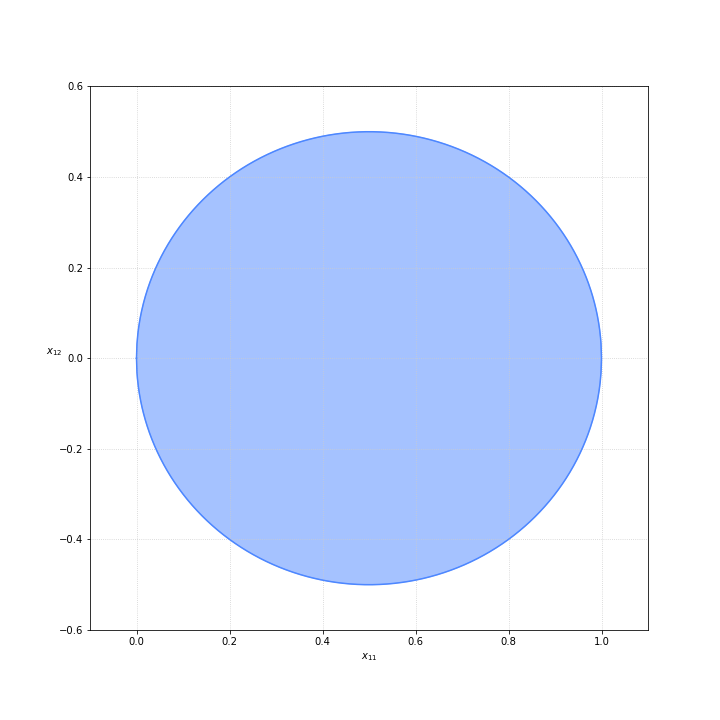
\includegraphics[width=0.5\textwidth]{img/ex3.png}   
    \caption{Přípustná množina řešení k úloze~\ref{eq:P3}.}
    \label{fig:ex3}
\end{figure}

\section{Dualita}

\subsubsection*{Duální úloha}

Podobně jako u lineárního programování použijeme Lagrangeovu dualitu k~odvození duální úlohy k \ref{eq:SDP-P}. Lagrangeova funkce je ve tvaru
$$
    L(X, \lambda, Z) = \langle C, X \rangle - \sum_{i=1}^m \lambda_i \left( \langle A_i, X \rangle - b_i \right) - \langle Z, X \rangle.
$$

\noindent K ní duální funkce
$$
    d(\lambda, Z) = \inf_{X \in S^n} L(X, \lambda, Z) = 
    \begin{cases}
        \lambda^T b & \dots\ C - \sum_{i=1}^m \lambda_i A_i - Z = 0, \\
        -\infty     & \dots\ \text{jinak.}
    \end{cases}
$$

\noindent Duální funkci použijeme v duální úloze
\begin{equation}\tag{SDP-D}
    \sup\left\{ \lambda^Tb \mid C - \sum_{i=1}^m \lambda_i A_i \succeq 0 \right\},
    \label{eq:SDP-D}
\end{equation}
kde $\lambda = (\lambda_1, \dots, \lambda_m)$ je duální proměnná.

\noindent Dostali jsme duální úlohu~\ref{eq:SDP-D} k úloze~\ref{eq:SDP-P}.

\subsubsection*{Slabá dualita semidefinitního programování}

Vztah mezi primární a duální úlohou je stejně jako u lineárního programování takový, že řešení jedné úlohy lze použít jako odhad na úlohu druhou. Nechť $X$ je libovolné přípustné řešení primární úlohy a $y$ je libovolné přípustné řešení duální úlohy. Potom
\begin{equation}
    \langle C, X \rangle - b^T y =
    \langle C, X \rangle - \sum_{i=1}^m y_i \langle A_i, X \rangle =
    \left\langle C - \sum_{i=1}^m A_i y_i, X \right\rangle \geq 0.
    \label{eq:weak_duality_SDP}
\end{equation}
Za pozornost stojí poslední nerovnost, která plyne z toho, že skalární součin dvou pozitivně semidefinitních matic je nezáporný. Odvození je následující. Mějme dvě matice $S, T \succeq 0$. Matici $S$ můžeme napsat jako součet \uv{rank one} matic. Označme $r_S = \textbf{rank}\ S$, tj.
$$
    S = \sum_{i=1}^{r_S} S_i = \sum_{i=1}^{r_S} \lambda_i s_i s_i^T.
$$
Dále se podíváme na součin $T \cdot S_i$. Tedy pro $i = 1, \dots, r_S$ platí
$$
    T \cdot S_i = \lambda_i s_i^T T s_i \geq 0,
$$
kde nerovnost plyne z toho, že matice $T$ je pozitivně semidefinitní.

O nerovnosti~\ref{eq:weak_duality_SDP} se mluví jako o slabé dualitě semidefinitního programování.

\subsubsection*{Silná dualita semidefinitního programování}

\begin{vt2}[podmínka optimality]
    Nechť $X$ je přípustné řešení úlohy~\ref{eq:SDP-P} a~$y$ je přípustné řešení úlohy~\ref{eq:SDP-D} taková, že splňují podmínku (komplementární skluzovosti)
    $$
        \left( C - \sum_{i=1}^m A_i y_i \right) X = 0.
    $$
    Potom $X$ je optimální řešení úlohy~\ref{eq:SDP-P} a $y$ je optimální řešení úlohy~\ref{eq:SDP-D}.
\end{vt2}

Obracená implikace sama o sobě neplatí, což znamená, že obecně dualitní rozdíl u semidefinitního programování není nulový. Musíme přidat podmínku kvalifikace omezení, kterou je například již zmíněná Slaterova podmínka. Ta je pro úlohu~\ref{eq:SDP-P} ve tvaru $X \succ 0$ a pro úlohu~\ref{eq:SDP-D} ve tvaru $C - \sum_i A_i y_i \succ 0$.

\begin{vt2}[silná dualita semidefinitního programování]
    Nechť úloha~\ref{eq:SDP-P} a úloha~\ref{eq:SDP-D} jsou striktně přípustné. Potom dualitní rozdíl jejich optimálních řešení je nulový.
\end{vt2}


\section{Vektorové programování}

Mějme $n$ vektorových proměnných $v_1, \dots, v_n$ v $\mathbb{R}^n$. \textbf{Vektorový program} je problém optimalizace lineární funkce skalárních součinů $\langle v_i, v_j \rangle$, vzhledem k~lineárním omezením na tyto skalární součiny.

Nyní ukážeme, že vektorové programy jsou ekvivalentní semidefinitním programům. Nechť tedy $\mathcal{V}$ je vektorový program s vektorovými proměnnými $v_1, \dots, v_n$ v $\mathbb{R}^n$ a $\mathcal{S}$ je příslušný semidefinitní program s $n^2$ proměnnými $y_{ij}$, kde hodnota $y_{ij}$ odpovídá skalárnímu součinu $\langle v_i, v_j \rangle$. Matice $Y$ je navíc pozitivně semidefinitní. Potom platí následující věta.

\begin{vt2}\cite{approximation-algorithms}
    Vektorový program $\mathcal{V}$ je ekvivalentní semidefinitnímu programu $\mathcal{S}$.
\end{vt2}
